\begin{frame}{Blockdiagramm}
    \begin{figure}
        \includegraphics[width=0.78\textwidth]{../documentation/diagrams/blockdiagram.pdf}
    \end{figure}

    \onslide<2->{
        \begin{tikzpicture}[remember picture, overlay]
            \node at ([xshift=8.3cm, yshift=-2.6cm]current page.north west) {
                \includesvg[width=1cm]{graphics/icon_electrical.svg}
            };
        \end{tikzpicture}

        \begin{tikzpicture}[remember picture, overlay]
            \node at ([xshift=7.9cm, yshift=-6.4cm]current page.north west) {
                \includesvg[width=1cm]{graphics/icon_optical.svg}
            };
        \end{tikzpicture}
    }
\end{frame}

\begin{frame}{Konzept: Optischer Teil}
    \begin{figure}
        \includegraphics[width=0.9\textwidth]{../documentation/diagrams/konzept_signalpfad.pdf}
    \end{figure}

    \iconoptical
\end{frame}

\subsection{Schaltungen}

\begin{frame}{TDC Elektrisch}
    \begin{figure}
        \includegraphics[page=2, trim=80 330 750 310, clip, width=0.8\textwidth]{../documentation/attachments/schematic.pdf}
    \end{figure}

    \iconelectrical
\end{frame}

\begin{frame}{TDC Optisch}
    \begin{figure}
        \includegraphics[page=2, trim=530 330 300 310, clip, width=0.8\textwidth]{../documentation/attachments/schematic.pdf}
    \end{figure}

    \iconoptical
\end{frame}

\begin{frame}{Laser Treiber}
    \begin{figure}
        \includegraphics[page=3, trim=100 520 550 60, clip, width=0.95\textwidth]{../documentation/attachments/schematic.pdf}
    \end{figure}

    \iconoptical
\end{frame}

\begin{frame}{Photo Receiver}
    \begin{figure}
        \includegraphics[page=3, trim=100 240 600 340, clip, width=0.9\textwidth]{../documentation/attachments/schematic.pdf}
    \end{figure}

    \iconoptical
\end{frame}

\begin{frame}{3D View}
    \begin{figure}
        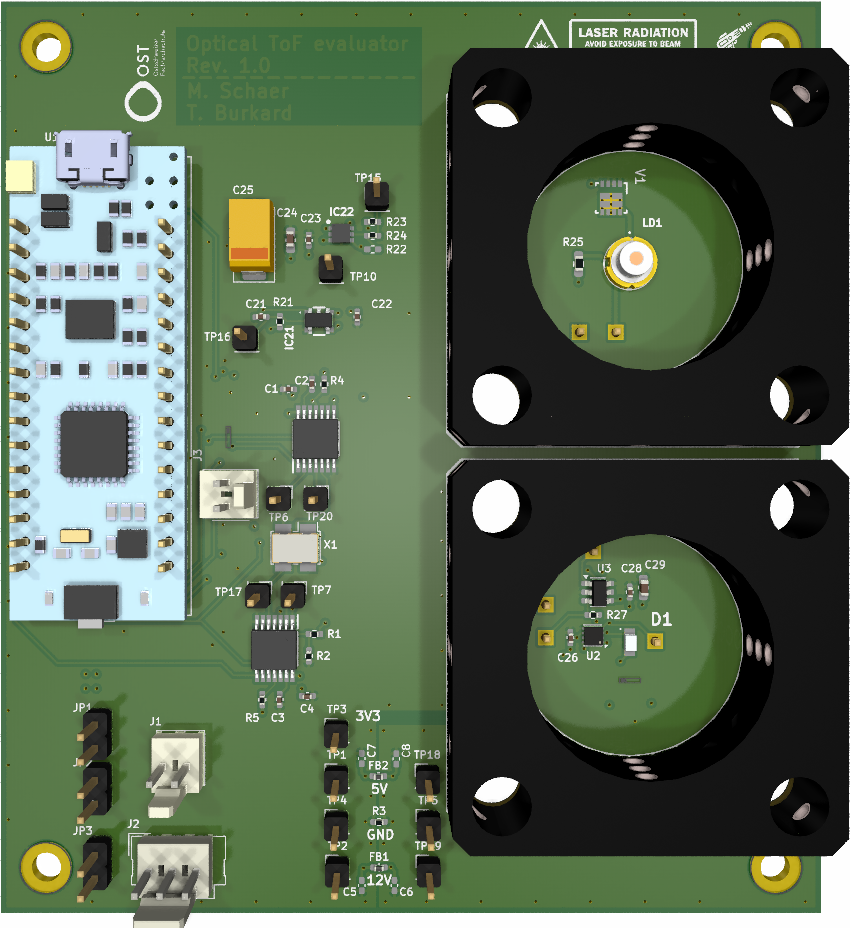
\includegraphics[width=0.4\textwidth]{../documentation/graphics/3d_top.png}
    \end{figure}
\end{frame}

\begin{frame}{Demonstrator}
    \begin{figure}
        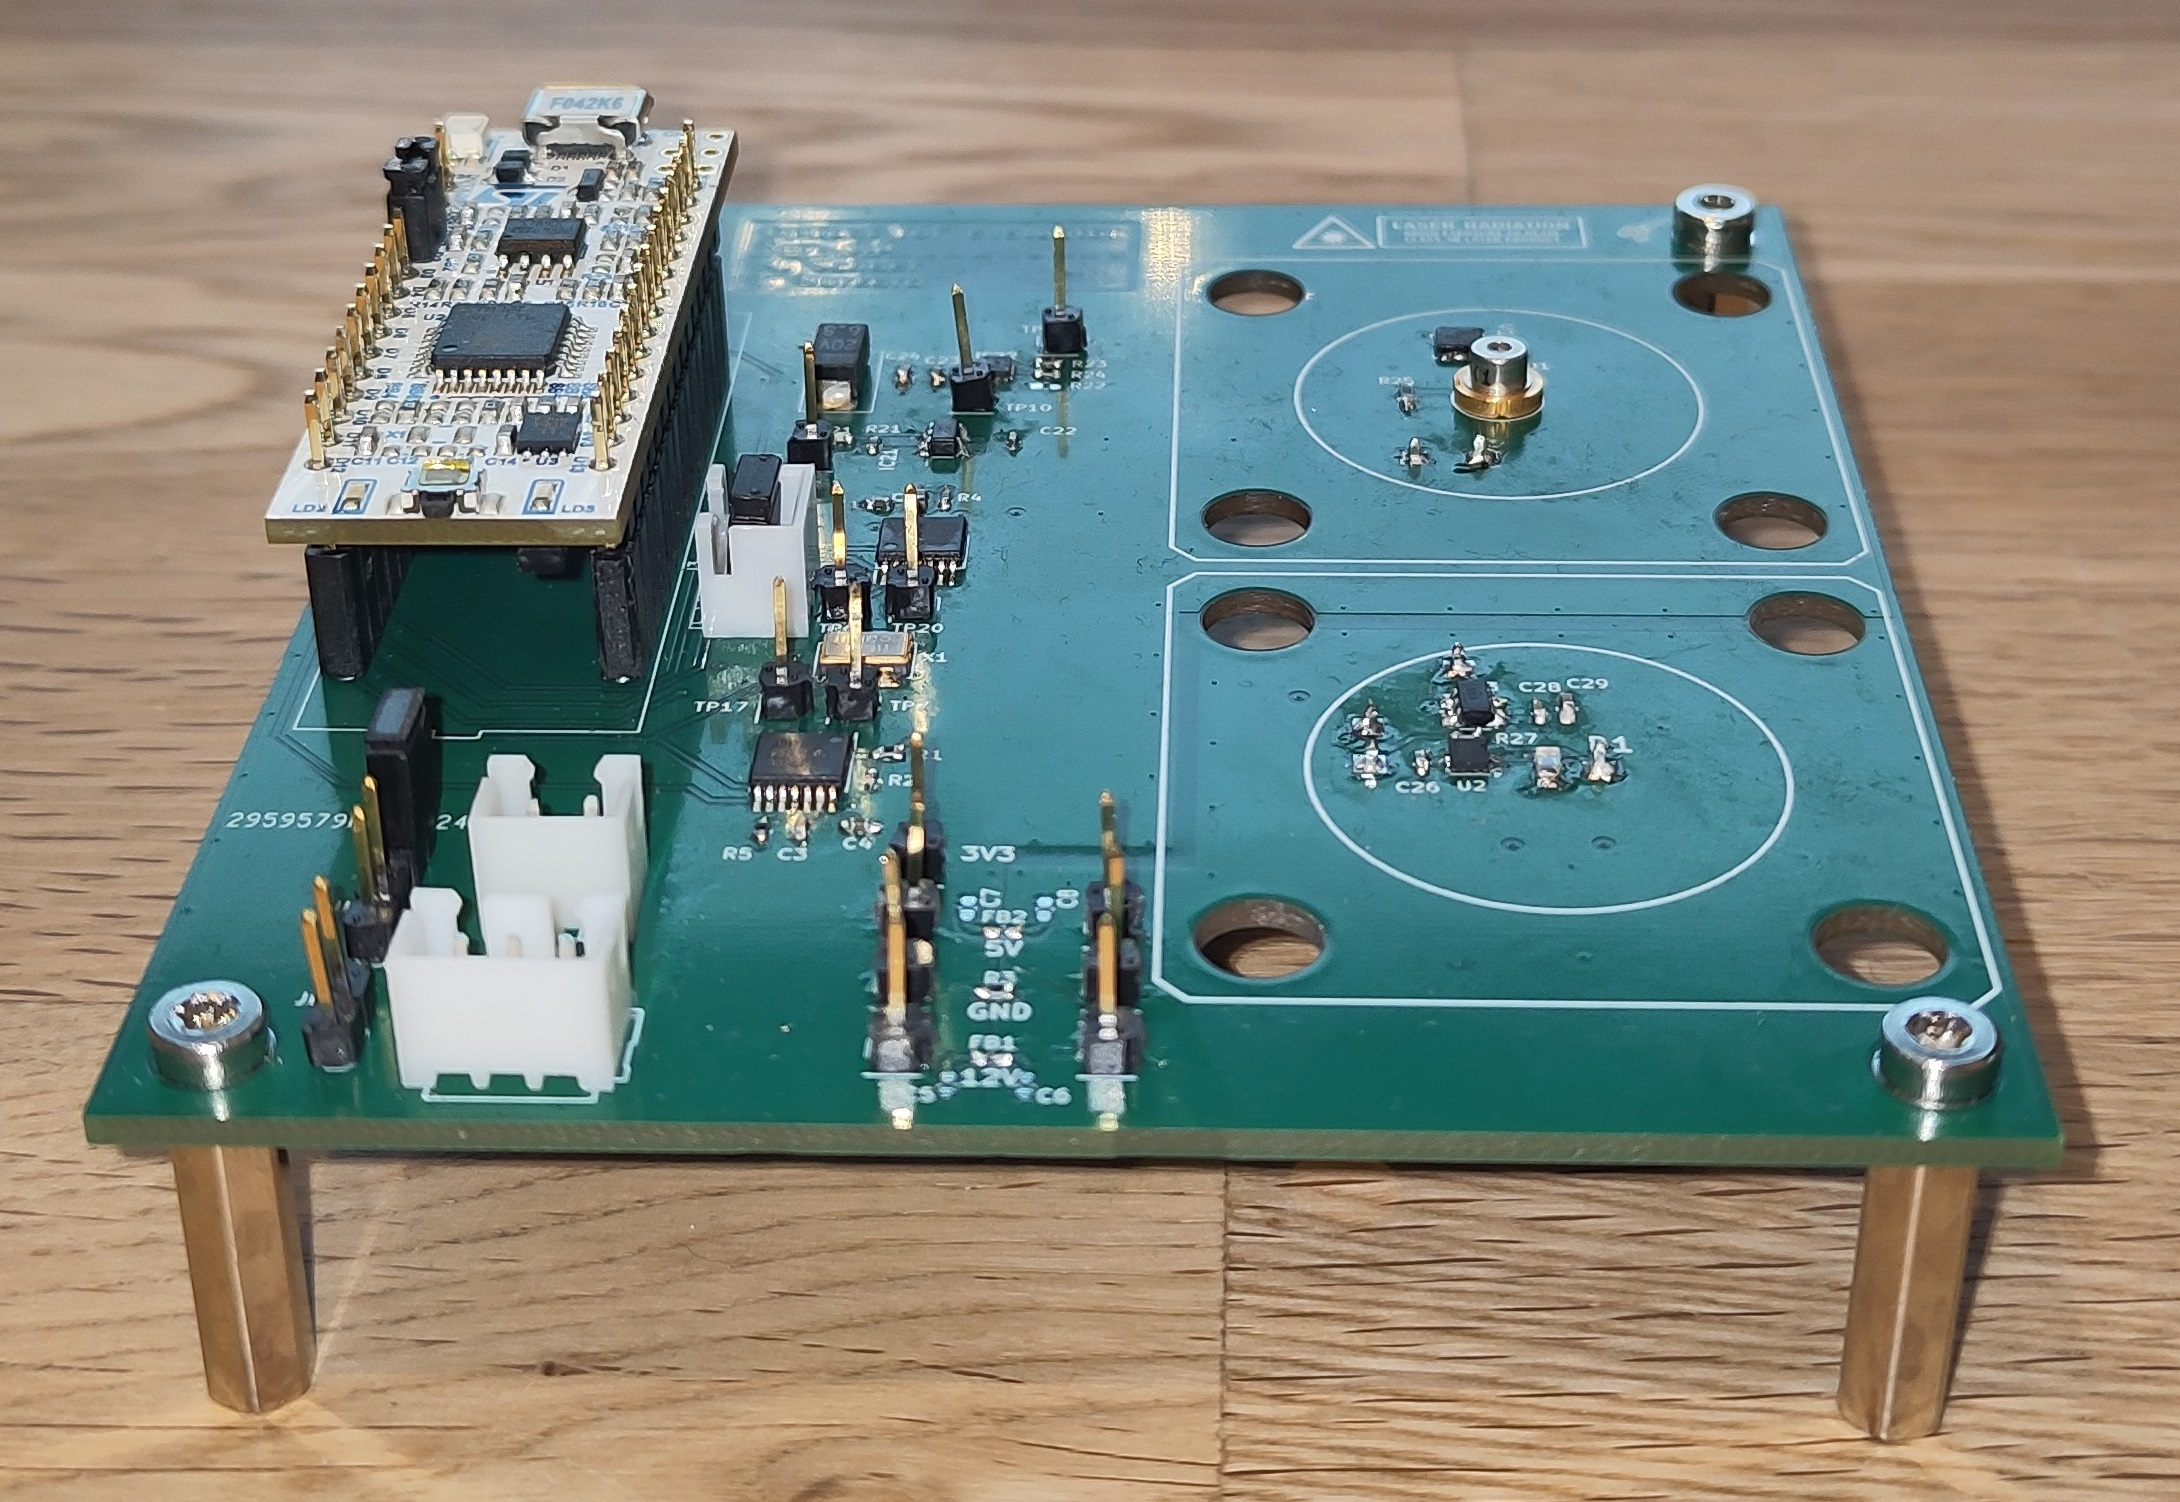
\includegraphics[width=0.6\textwidth]{../documentation/graphics/photo_demonstrator_front_wo_lens.jpg}
    \end{figure}
\end{frame}

\subsection{Firmware}

\begin{frame}{Firmware Blockdiagramm}
    \begin{figure}
        \includegraphics[width=0.55\textwidth]{../documentation/diagrams/Aufbau_FW.pdf}
    \end{figure}
\end{frame}

\begin{frame}{Firmware Beispiel: Konfiguration}
    \only<1>{\codehighlight{C}{1}{99}{sourcecode/tdc_example_config.c}}
    \only<2>{\codehighlight{C}{1}{5}{sourcecode/tdc_example_config.c}}
    \only<3>{\codehighlight{C}{7}{13}{sourcecode/tdc_example_config.c}}
\end{frame}

\begin{frame}{Firmware Beispiel: Messung}
    \only<1>{\codehighlight{C}{1}{99}{sourcecode/tdc_example_measure.c}}
    \only<2>{\codehighlight{C}{4}{4}{sourcecode/tdc_example_measure.c}}
    \only<3>{\codehighlight{C}{6}{8}{sourcecode/tdc_example_measure.c}}
    \only<4>{\codehighlight{C}{10}{10}{sourcecode/tdc_example_measure.c}}
    \only<5>{\codehighlight{C}{12}{12}{sourcecode/tdc_example_measure.c}}
\end{frame}
